\documentclass{beamer}
%\documentclass[handout]{beamer}
%\documentclass[handout, notes=show]{beamer}

\usepackage[french]{babel}
\usepackage[utf8]{inputenc}
\usepackage{times}
\usepackage[T1]{fontenc}

\usepackage{graphicx}
\graphicspath{{../report/img/}{./img/}}
\usepackage{hyperref}
\hypersetup{colorlinks=true,linkcolor=red}
\usepackage{pgfpages}

\mode<presentation>
{
    % Complete themes
    %\usetheme{default}
    %\usetheme{Bergen}
    %\usetheme{Boadilla}
    %\usetheme{CambridgeUS}
    %\usetheme{Antibes}
    %\usetheme{Berkeley}
    %\usetheme{Warsaw}
    %\usetheme{Singapore}
    %\usetheme{Berlin}
    %\usetheme{Copenhagen}

    % Inner themes
    %\useinnertheme{default}
    %\useinnertheme{circles}
    %\useinnertheme{rectangles}
    \useinnertheme[shadow]{rounded}
    %\useinnertheme{inmargin}

    % Outer themes
    \useoutertheme{default}
    %\useoutertheme{infolines}
    %\useoutertheme{miniframes}
    %\useoutertheme{smoothbars}
    %\useoutertheme{sidebar}
    %\useoutertheme{split}
    %\useoutertheme{shadow}
    %\useoutertheme{tree}
    %\useoutertheme{smoothtree}

    % Complete color themes
    %\usecolortheme{albatross}
    %\usecolortheme{beetle}
    %\usecolortheme{crane}
    %\usecolortheme{dove}
    %\usecolortheme{fly}
    %\usecolortheme{monarca}
    %\usecolortheme{seagull}
    %\usecolortheme{wolverine}
    %\usecolortheme{beaver}
    %\usecolortheme{spruce}

    % Inner color themes
    \usecolortheme{lily}
    %\usecolortheme{orchid}
    %\usecolortheme{rose}

    % Outer color themes
    \usecolortheme{whale}
    %\usecolortheme{seahorse}
    %\usecolortheme{dolphin}

    % Special purpose color theme
    %\usecolortheme{default}
    \usecolortheme[named=darkgray]{structure}
    %\usecolortheme{sidebartab}

    % Set colors
    %\hypersetup{colorlinks=true,linkcolor=red}

    \beamertemplatenavigationsymbolsempty
    \setbeamercovered{transparent=10}
    %\setbeamertemplate{footline}[frame number]
    \setbeamertemplate{footline}
    {
        \hfill \footnotesize{\insertframenumber/\inserttotalframenumber} \hspace{0.5cm}
        \vspace{0.5cm}
    }
}

\title[]{Mathématiques discrètes}
\subtitle{Blackjack}
\author{Claudio Sousa, David Gonzalez}
\institute{HEPIA}
\date{21/06/2018}

\pgfdeclareimage[width=1cm]{logo}{logo}
\logo{\pgfuseimage{logo}}

\setcounter{tocdepth}{3}

\begin{document}

\begin{frame}[plain]
    \titlepage
\end{frame}

\section{Catégorisation}

\begin{frame}
    \frametitle{Catégorisation}
\end{frame}

\section{Tests empiriques}

\begin{frame}
    \frametitle{Tests empiriques: Chance du joueur avec stratégie basique}
    \begin{figure}[H]
        \begin{center}
            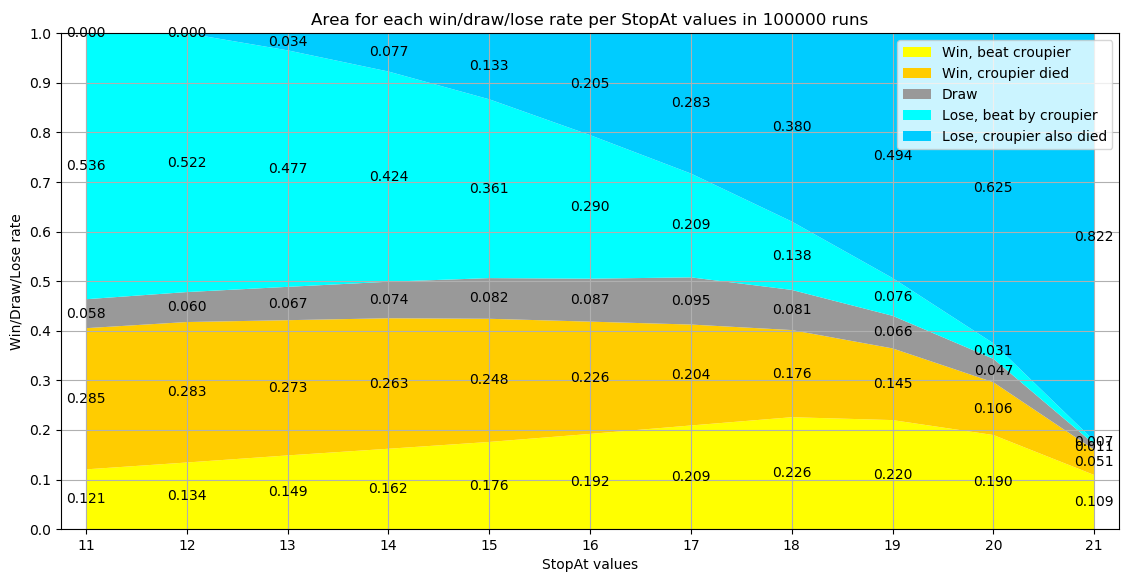
\includegraphics[width=1\textwidth]{empirical_graph1}
        \end{center}
    \end{figure}
\end{frame}

\begin{frame}
    \frametitle{Tests empiriques: Chance du joueur par main initial du croupier}
    \begin{figure}[H]
        \begin{center}
            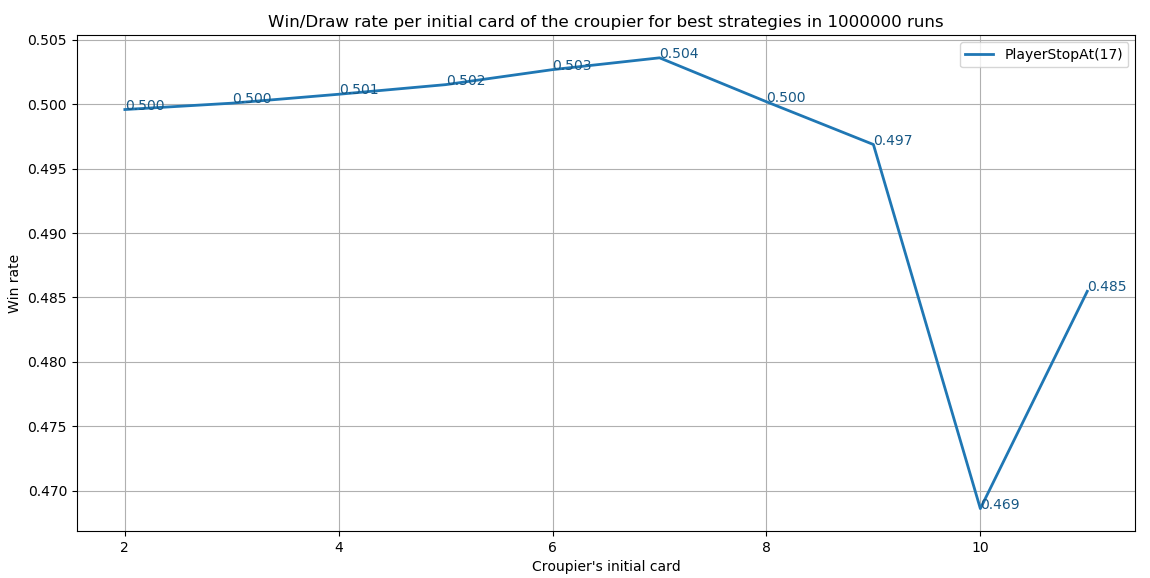
\includegraphics[width=1\textwidth]{empirical_graph2}
        \end{center}
    \end{figure}
\end{frame}

\begin{frame}
    \frametitle{Tests empiriques: Chance du joueur avec des stratégies différentes}
    \begin{figure}[H]
        \begin{center}
            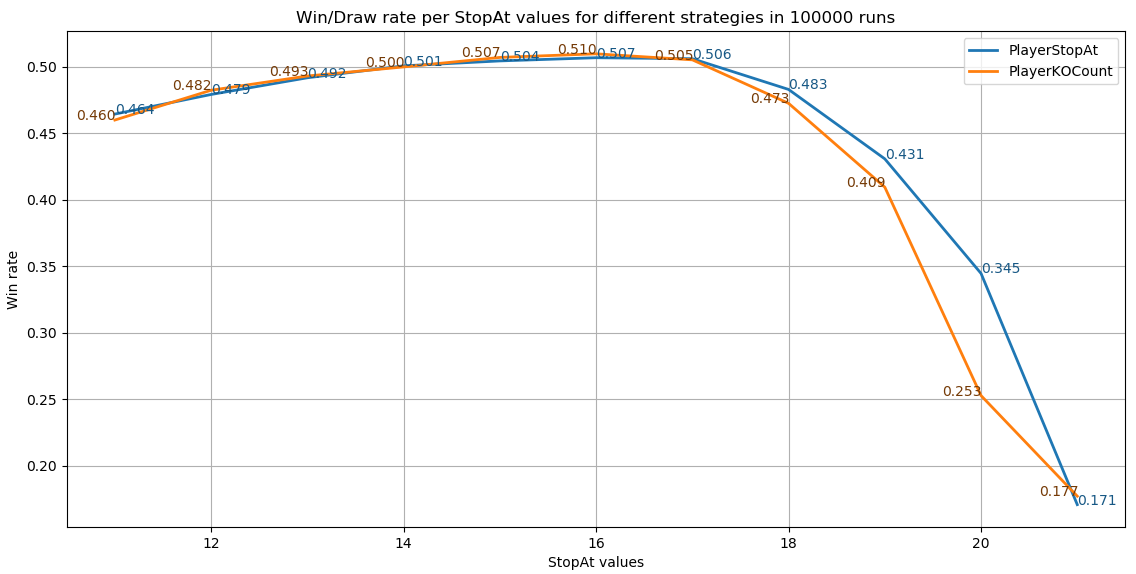
\includegraphics[width=1\textwidth]{empirical_graph3}
        \end{center}
    \end{figure}
\end{frame}

\section{Théorie}

\begin{frame}
    \frametitle{Théorie: Chance du croupier}
    \begin{figure}[H]
        \begin{center}
            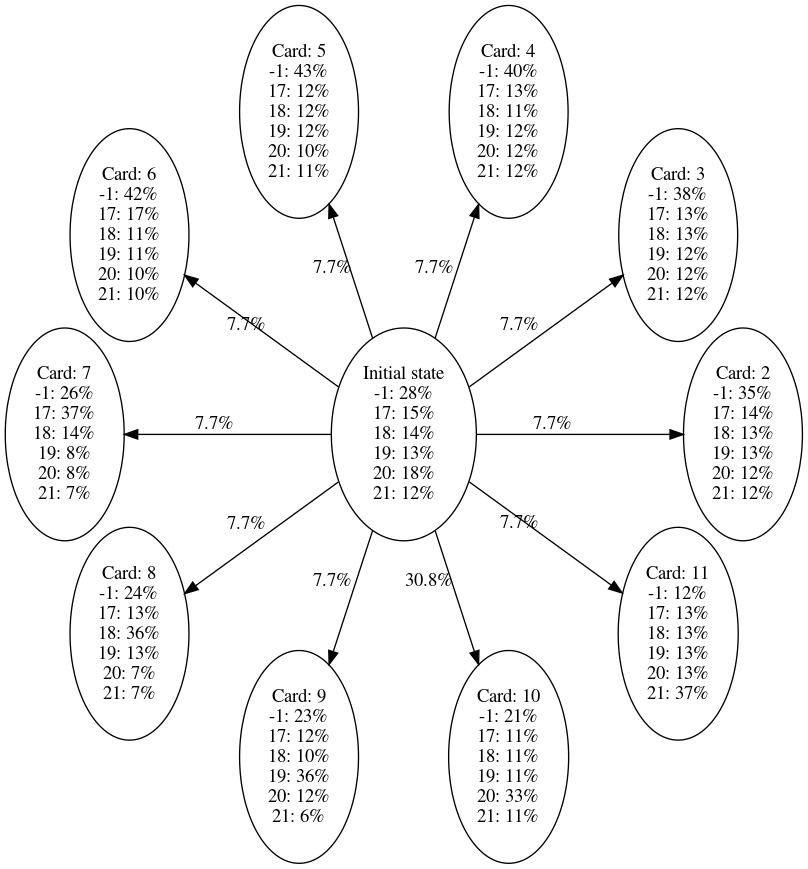
\includegraphics[width=0.7\textwidth]{theoretical_croupier}
        \end{center}
    \end{figure}
\end{frame}

\begin{frame}
    \frametitle{Théorie: Chance du joueur}
    \begin{figure}[H]
        \begin{center}
            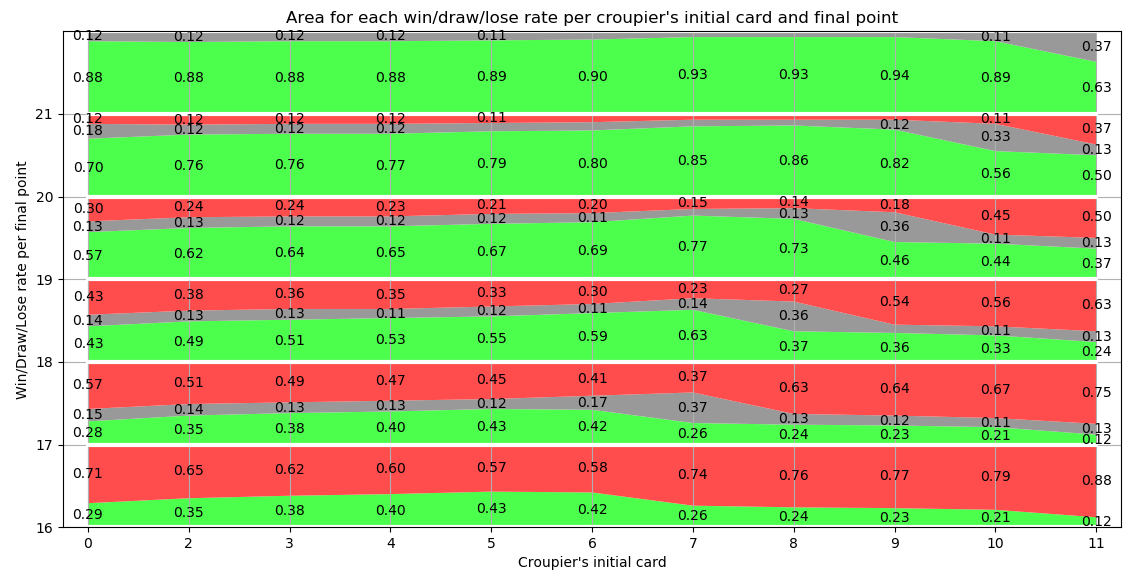
\includegraphics[width=1\textwidth]{theoretical_graph1}
        \end{center}
    \end{figure}
\end{frame}

\end{document}
